\chapter{Un profil UML pour aider à la rédaction d'un GDD}
\label{game-genesis.sect}
%GDD
Le \emph{Game Design Document}, comme décrit dans la Section~\ref{sect.GDD}, permet de réunir toutes les informations de design nécessaires au développement d'un jeu vidéo. La structure du GDD est définit par des bonnes pratiques et selon les besoins de design du jeu concerné.

%MDA
Le \emph{Framework Mechanics, Dynamics, Aesthetics}, comme décrit dans le Chapitre~\ref{chap.MDA}, permet de séparer les différents aspects du design d'un jeu vidéo. L'aspect \emph{Mechanics} permet de représenter tous les éléments du jeu, les Dynamics décrivent le comportement des \emph{Mechanics} et l'Aesthetics sont les émotions découlant des Dynamics que le jeu génère chez le joueur.

%UML
Les profils UML, décrit dans le Chapitre~\ref{chap.profils-UML}, permettent d'étendre les objets présents dans UML. Mettre en place un profil UML permet d'adapter le modèle et son contenu à un domaine particulier. Un profil se compose de stéréotypes, de valeurs étiquetés et de contraintes afin de pouvoir ajouter les modifications sur les éléments des modèles.


\section{\emph{Game Genesis} un profil pour la modélisation d'un \emph{Game Design Document} }
\label{sect.gg_what}
%quoi
Game Genesis est un profil UML permettant d'adapter UML au domaine du design de jeu vidéos. 
Plus précisément Game Genesis adapte le diagramme de classes UML afin de l'adapter à la rédaction d'un GDD.

Afin de rédiger un GDD un \emph{Game designer} doit d'abord définir les bases du jeu.
Durant cette étape le \emph{game designer} va devoir définir un certain nombre de \emph{Mechanics} qui correspondent aux objets présents dans le jeu ainsi que leurs actions et interactions.
Ces \emph{Mechanics} peuvent aussi bien être des objets visibles dans le jeu comme des personnages, des ennemis, des armes, des bâtiments mais également des mécaniques autour du jeu comme des cartes, des chronomètres, des statistiques, etc.
Toutes ces \emph{Mechanics} ont des caractéristiques communes et des caractéristiques qui leur sont propres.

%comment
Game Genesis est un profil UML qui permet à un \emph{game designer} de répertorier et décrire ces \emph{Mechanics} sous forme de diagrammes de classes.
Chaque catégorie de \emph{Mechanics} est représenté par une classe.
Chaque \emph{Mechanics} est représenté par une classe.
L'appartenance des \emph{Mechanics} à une catégorie est définie par les notions d'héritage.
Les caractéristiques des catégories et des \emph{Mechanics} sont représentées par les attributs des classes.
Les interactions sont représentées par des associations entre les classes.

%pourquoi
Un diagramme de classes UML apporte beaucoup d'avantages dans la modélisation des \emph{Mechanics}.
\begin{itemize}
    \item Structure
    \item Langage de modélisation formel et normalisé
    \item Support de communication performant
    \item Encourage l'utilisation d'outils adaptés
    \item Facilement versionnable
    \item Est assez souple pour s'adapter
\end{itemize}

Cependant UML est un langage avant tout destiné à modéliser les systèmes informatiques et les processus d'affaire. 
Il est alors nécessaire de l'adapter afin de lui apporter le vocabulaire et les logiques nécessaires à la description de \emph{Mechanics} dans un jeu vidéo.
C'est à cela que sert un profil UML.
   




\section{Game Genesis en détail}
\begin{figure}[H]
    \begin{adjustbox}{width=\linewidth}
        \begin{forest}
         [Model
         [Item
             [Wearable
                 [Weapon,tier=before
                    [Fig.~\ref{A-Weapon}]
                 ]
                 [Equipment,tier=before
                    [Fig.~\ref{A-Equipment}]
                 ]
                 [Jewerly,tier=before
                    [Fig.~\ref{A-Jewerly}]
                 ]
                 [Tool,tier=before
                    [Fig.~\ref{A-Tool}]
                 ]
             ]
             [Add-on,tier=before
                    [Fig.~\ref{A-Add-on},tier=bottom]
             ]
             [Usable,tier=before
                    [Fig.~\ref{A-Usable},tier=bottom]
             ]
             [Craft,tier=before
                    [Fig.~\ref{A-Craft},tier=bottom]
            ]
             [Currency,tier=before
                    [Fig.~\ref{A-Currency},tier=bottom]
            ]
         ]
         ]
        \end{forest}
    \end{adjustbox}
    \caption{Arbre des stéréotypes de Game Genesis}
    \label{fig.GG}
\end{figure}
    
\begin{figure}[H]
    \begin{adjustbox}{width=\linewidth}
        \begin{forest}
         [Model
         [Animate Fig.\ref{A-Animate},tier=bottom]
         [CharacterSheet,tier=before
                [Fig.~\ref{A-Statistic},tier=bottom]
                [Fig.~\ref{A-Attribute},tier=bottom]
                [Fig.~\ref{A-Information},tier=bottom]
         ]
         [Lore Fig.~\ref{A-Lore},tier=bottom]
         [World Fig.~\ref{A-World},tier=bottom]
         [Interaction Fig.~\ref{A-Interaction},tier=bottom]
         ]
        \end{forest}
    \end{adjustbox}
    \caption{Arbre des stéréotypes de Game Genesis (suite)}
    \label{fig.GG2}
\end{figure}

\subsection{Stéréotypes}
Dans la Section \ref{sect.uml.ster} nous avons décris le mécanisme de redéfinition d'objets UML par les Stéréotypes. 
Dans \emph{Game Genesis} nous faisons usage des stéréotypes afin de redéfinir les classes d'un modèle et ainsi l'adapter pour la rédaction de GDD.
Dans l'article de Salazar \emph{et al.}~\cite{GDD_software}, plus particulièrement la documentation additionnelle de cet article \cite{salazar_gdd}, nous avons identifié un certain nombre de \emph{Mechanics} présentes dans le GDD.
Nous avons constaté que tous les éléments étaient répartis dans des catégories possédant elles-mêmes des caractéristiques.
Nous avons extrait les catégories suivantes :
\begin{itemize}
    \item Player Character
    \item Non Player Character
    \item Enemy
    \item Final Enemy
    \item Help Object
    \item Extra Object
    \item Other Object
\end{itemize}

Les classes UML fonctionnent avec un systéme d'héritage de classes.
La classe enfant hérite des attributs et méthodes de la classe parent.
Dans un GDD les \emph{Mechanics} héritent des attributs énoncés dans les catégories
Une fois chaque \emph{Mechanics} de jeu définies les attributs des catégories étaient spécifiés dans les \emph{Mechanics}.
Cela fonctionne de la même manière qu'un héritage de classe.


C'est ainsi que nous avons décidé d'utiliser un diagramme de classes afin de représenter les \emph{Mechanics} comme des classes et de spécifier leurs caractéristiques dans les attributs.
Nous présentons un exemple d'héritage présent dans le profil UML dans la Fig.~\ref{fig.herit}.

\begin{figure}[H]
    \centering
    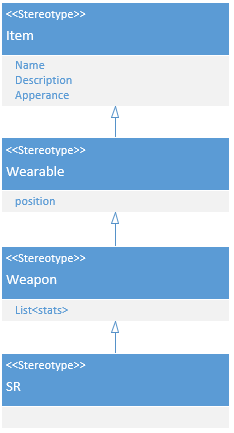
\includegraphics[width=5cm]{10_img/chap5/heritage.PNG} 
    \caption{Représentation de l'héritage imposé à un objet "SR" (\emph{Sniper Rifle})}
    \label{fig.herit}
\end{figure}

Dans la Fig.~\ref{fig.sniper} nous proposons un exemple d'une classe Sniper1, étant un objet de \emph{Mechanics} du GDD utilisant \emph{Game Genesis}.
Nous voyons que la classe hérite ainsi des attributs des Stéréotypes précédents dans la logique d'héritage de classes.
\begin{figure}[H]
    \centering
    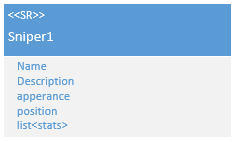
\includegraphics[width=5cm]{10_img/chap5/sniper.PNG} 
    \caption{Exemple d'un objet Sniper1 héritant du stéréotype "SR" (\emph{Sniper Rifle})}
    \label{fig.sniper}
\end{figure}



\subsection{Interaction}
Les éléments de \emph{Mechanics} ne sont cependant pas tous des éléments isolés et une expérience de jeu ne serait rien sans l'interaction que le joueur peut avoir avec son environnement.
Ces interactions sont présentées dans le template de GDD de Salazar \emph{et al.}~\cite{salazar_gdd} sous forme de règles d'interaction.
Ces règles sont composées de plusieurs éléments :
\begin{itemize}
    \item Deux (ou plus) \emph{Mechanics} 
    \item Une interaction entre ces \emph{Mechanics}
    \item Une contrainte appliquée à cette interaction (optionnelle)
\end{itemize}
Les interactions sont disponibles dans la Figure~\ref{A-Interaction}.

\section{Conclusion}


%%%%%%%%%%%%%%%%%%%%%%%%%%%%%%%%%%%%%%%%%%%%%%%%%%%%%%%%%%%%%%%%%%%%%%%%%%
\begin{comment}
\chapter{Un langage de modélisation pour l'établissement d'un Game Design Document}

\section{Le concept}
\subsection{Définition}
\subsubsection{Quoi ?}
Un langage permettant de modéliser et stocker des idées lors des phases de Breakthrough et de Conception d'un projet de jeu vidéo. La modélisation peut être graphique et/ou textuelle avec application des modifications en parallèle. \\
Les informations peuvent contenir tout le nécessaire pour exprimer les idées (textes, informations numériques, chemins de fichiers...). Les champs peuvent être personalisables pour permettre de la souplesse aux utilisateurs.

\subsubsection{Pour quoi faire ?}
\paragraph{Des outils de modélisation existent pour tous les domaines reliés au développement de logiciels. Ils sont souvent spécifiques à un corps de métier afin de pouvoir proposer un maximum de fonctionnalités spécifiques sans devenir trop compliqué et en utilisant un vocabulaire précis qui correspond au corps de métier concerné.}

\paragraph{Il y a peu ou pas de langages de modélisation plus généraux pour des domaines multi-métiers. Le but est de pouvoir modéliser la réflexion créative en fournissant un élément visuel permettant de mind-mapper les idées, les stocker et les réutiliser. \\
Il faut que la modélisation soit assez souple pour pouvoir répondre aux besoins de chacun des corps de métier d'où le fait que les éléments et attributs peuvent avoir des identifiants spécifiques définis librement par l'utilisateur.}

\subsubsection{Pour quelles raisons ?}
\paragraph{Les supports de réflexion actuellement utilisés : cahier des charges, réunions, notes écrites, mails, minds-maps... L'organisation de ces différents supports dans un ensemble cohérent est tr;s compliqué. Dans un cahier des charges il est compliqué de classer les idées à la volée. Un mind-map nécessite une numérisation ou une retranscription sur un outil de mind-mapping qui sont toutes les deux des techniques non péreines et risquées dans la conservation des données. Des notes écrites peuvent se perdre et n'ont pas de durabilité sur le long terme. Des mails sont péreins mais il est difficile de les organiser pour le stockage de l'information.}
\paragraph{Un langage de modélisation graphique et textuel permettrait de mind-mapper les idées à la volée sous forme de cubes contenant les données nécessaires. La hiérarchisation des éléments permettrait de gérer des héritages et des relations ainsi que d'éviter la répétition trop abondante des mêmes informations. Les faces des cubes permettrait d'isoler les informations nécessaires à chacun des corps de métier.}
\end{comment}
